
\section{Introduction}

Reinforcement learning (RL) is an area of research focusing on finding an action that will maximize a reward function given the state of an agent. Finding the optimal state action value requires large amounts exploration of the environment. The ability to gather reliable data is crucial to the learning process because this provides the learning algorithm with an accurate representation of how the state evolves with a given action. 

RL has recently become a topic of interest due to its ability to solve problems without knowledge of the underlying dynamics.This model free approach is used over a large set of applications including control theory, natural language processing, image recognition, and medical diagnoses. A very popular model-free reinforcement learning algorithm is Q-learning which operates by applying incremental estimation to the Bellman equation\cite{DMU}.

\vspace{-6mm}
\begin{equation}
	Q(s,a) \leftarrow Q(s,a)+\alpha(r + \gamma \max_{a'} Q(s',a') - Q(s,a))
\end{equation}
\vspace{-8mm}

The game we would like to investigate, Super Smash Bros Melee, presents an environment complex dynamics an a continuous state space that would be infeasible to represent as discrete values. A model-free approach eliminates the need for a state transition model and generalization allows the agent to approximate the optimal action at a given state. Given the nature of the problem, we chose to implement a perceptron Q-learning algorithm. In this algorithm, a set of weights for each action $\theta_a$ is trained on a basis function $\beta(s)$, such that the state-action value can be globally approximated as $Q(s,a) = \theta^T_a\beta(s)$. The action weights are trained in a batch learning process after each game.

\vspace{-6mm}
\begin{equation}
	\theta_a \leftarrow \theta_a+\alpha(r + \gamma \max_{a'} \theta_{a'}^T\beta(s',a') -  \theta_{a}^T\beta(s,a))\beta(s,a)
\end{equation}
\vspace{-8mm}

Super Smash Bros Melee is a platform based fighting game in which the goal is to knock your opponent off of the stage. Damage dealt to the opponent increases the distance they fly when hit. A winning strategy in the game involves dealing damage to the opponent and subsequently knocking them off the stage while simultaneously avoiding the opponents attempts to do the same. While the game has many available characters and stages, we limited the project to a single stage (Final Destination) and character (Captain Falcon) for convenience of training, although the work done is general and allows for training of any character and stage combination.

\begin{figure}[!htb]
\centering
	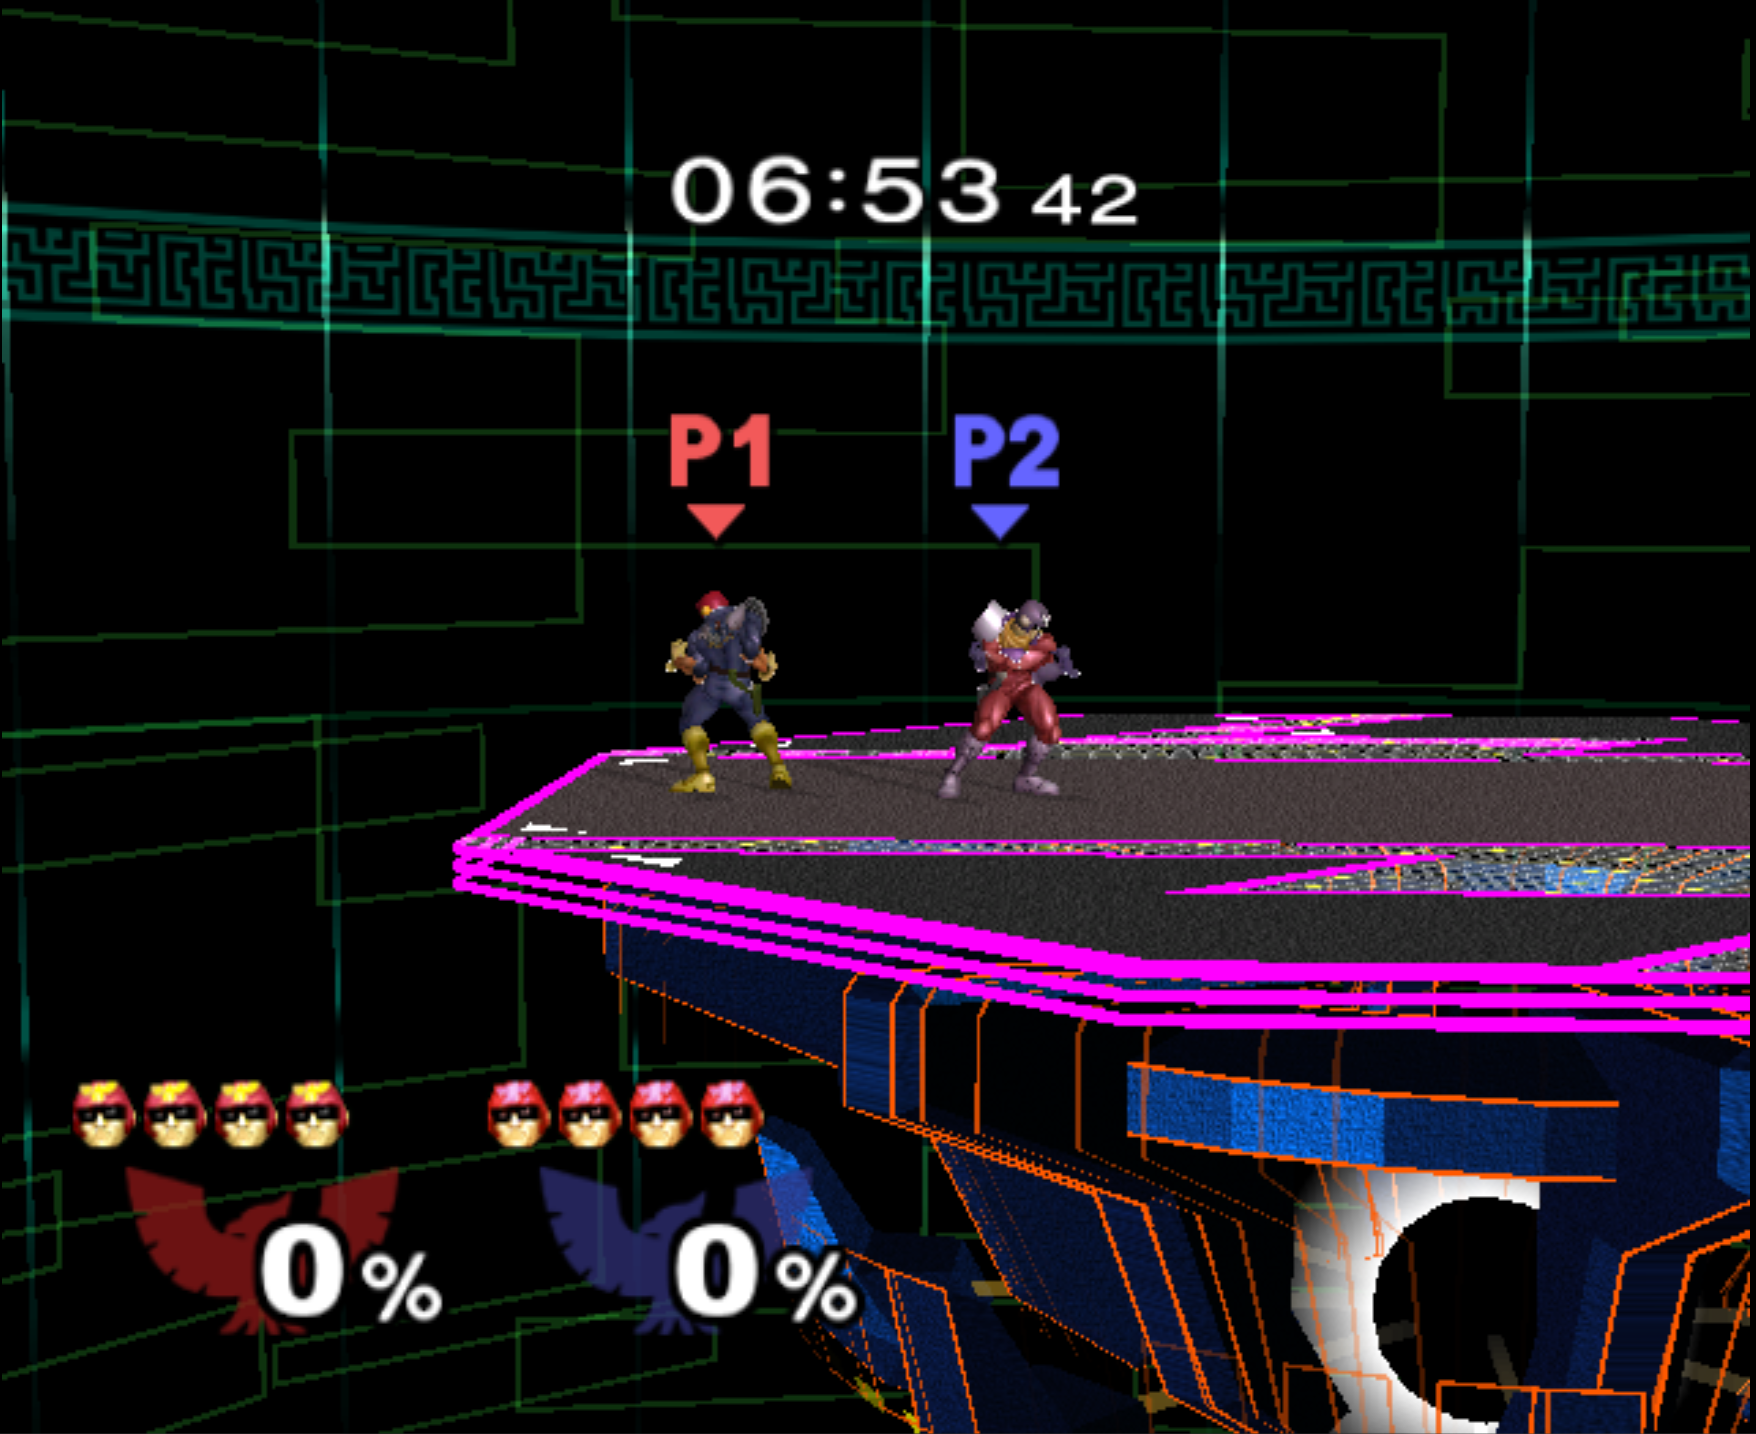
\includegraphics[width=70mm]{stage.png}
	\caption{Super Smash Brothers Melee game environment. \label{melee}}
\end{figure}

To interact with the game environment, we leverage the open-source game emulator Dolphin and an python library libmelee which provides an interface for reading state values and sending controller inputs to the agent. 

%We define the action space as $\mathbb{A}$ and the state space as $\mathbb{S}$. The action space contains a set of actions that are mapped to a combination of buttons being pressed on a gamecube controller. The state space contains a set of continuous and discrete variables that represent the agent and its opponent in the environment. Values encoded in the basis function $\beta(s)$ from the state space include the agents position, relative position to the opponent, current animation value, damage levels, direction facing, and number of jumps remaining.






